%% March 2018
%%%%%%%%%%%%%%%%%%%%%%%%%%%%%%%%%%%%%%%%%%%%%%%%%%%%%%%%%%%%%%%%%%%%%%%%%%%%
% AGUJournalTemplate.tex: this template file is for articles formatted with LaTeX
%
% This file includes commands and instructions
% given in the order necessary to produce a final output that will
% satisfy AGU requirements, including customized APA reference formatting.
%
% You may copy this file and give it your
% article name, and enter your text.
%
%
% Step 1: Set the \documentclass
%
% There are two options for article format:
%
% PLEASE USE THE DRAFT OPTION TO SUBMIT YOUR PAPERS.
% The draft option produces double spaced output.
%

%% To submit your paper:
\documentclass[draft]{agujournal2018}
\usepackage{apacite}
\usepackage{url} %this package should fix any errors with URLs in refs.
\usepackage{lineno}
\linenumbers
%%%%%%%
% As of 2018 we recommend use of the TrackChanges package to mark revisions.
% The trackchanges package adds five new LaTeX commands:
%
%  \note[editor]{The note}
%  \annote[editor]{Text to annotate}{The note}
%  \add[editor]{Text to add}
%  \remove[editor]{Text to remove}
%  \change[editor]{Text to remove}{Text to add}
%
% complete documentation is here: http://trackchanges.sourceforge.net/
%%%%%%%

\draftfalse

%% Enter journal name below.
%% Choose from this list of Journals:
%
% JGR: Atmospheres
% JGR: Biogeosciences
% JGR: Earth Surface
% JGR: Oceans
% JGR: Planets
% JGR: Solid Earth
% JGR: Space Physics
% Global Biogeochemical Cycles
% Geophysical Research Letters
% Paleoceanography and Paleoclimatology
% Radio Science
% Reviews of Geophysics
% Tectonics
% Space Weather
% Water Resources Research
% Geochemistry, Geophysics, Geosystems
% Journal of Advances in Modeling Earth Systems (JAMES)
% Earth's Future
% Earth and Space Science
% Geohealth
%
% ie, \journalname{Water Resources Research}

\journalname{Geophysical Research Letters}


\begin{document}

%% ------------------------------------------------------------------------ %%
%  Title
%
% (A title should be specific, informative, and brief. Use
% abbreviations only if they are defined in the abstract. Titles that
% start with general keywords then specific terms are optimized in
% searches)
%
%% ------------------------------------------------------------------------ %%

% Example: \title{This is a test title}

\title{Partitioning Thresholds in Hybrid Implicit-Explicit Representations of Naturally Fractured Reservoirs}

%% ------------------------------------------------------------------------ %%
%
%  AUTHORS AND AFFILIATIONS
%
%% ------------------------------------------------------------------------ %%

% Authors are individuals who have significantly contributed to the
% research and preparation of the article. Group authors are allowed, if
% each author in the group is separately identified in an appendix.)

% List authors by first name or initial followed by last name and
% separated by commas. Use \affil{} to number affiliations, and
% \thanks{} for author notes.
% Additional author notes should be indicated with \thanks{} (for
% example, for current addresses).

% Example: \authors{A. B. Author\affil{1}\thanks{Current address, Antartica}, B. C. Author\affil{2,3}, and D. E.
% Author\affil{3,4}\thanks{Also funded by Monsanto.}}

\authors{Daniel Wong\affil{1}, Florian Doster\affil{1}, Sebastian Geiger\affil{1}, Arjan Kamp\affil{2}}


% \affiliation{1}{First Affiliation}
% \affiliation{2}{Second Affiliation}
% \affiliation{3}{Third Affiliation}
% \affiliation{4}{Fourth Affiliation}

\affiliation{1}{Institute of Petroleum Engineering, Heriot-Watt University}
\affiliation{2}{Total S.A.}
%(repeat as many times as is necessary)

%% Corresponding Author:
% Corresponding author mailing address and e-mail address:

% (include name and email addresses of the corresponding author.  More
% than one corresponding author is allowed in this LaTeX file and for
% publication; but only one corresponding author is allowed in our
% editorial system.)

% Example: \correspondingauthor{First and Last Name}{email@address.edu}

\correspondingauthor{Daniel Wong}{dlw1@hw.ac.uk}

%% Keypoints, final entry on title page.

%  List up to three key points (at least one is required)
%  Key Points summarize the main points and conclusions of the article
%  Each must be 100 characters or less with no special characters or punctuation

% Example:
% \begin{keypoints}
% \item	List up to three key points (at least one is required)
% \item	Key Points summarize the main points and conclusions of the article
% \item	Each must be 100 characters or less with no special characters or punctuation
% \end{keypoints}

\begin{keypoints}
\item Small fractures up to a threshold size can be lumped with the rock matrix and upscaled into an equivalent porous medium.
\item We determine the threshold size from the relationship between upscaled permeability and the size range of small fractures.
\item Where applicable, the upscaled permeabilities are efficiently established using the Effective Medium Theory compared to numerical upscaling.
\end{keypoints}

%% ------------------------------------------------------------------------ %%
%
%  ABSTRACT
%
% A good abstract will begin with a short description of the problem
% being addressed, briefly describe the new data or analyses, then
% briefly states the main conclusion(s) and how they are supported and
% uncertainties.
%% ------------------------------------------------------------------------ %%

%% \begin{abstract} starts the second page

\begin{abstract}
Complex fracture patterns are simplified in this work using hybrid implicit-explicit representations. Hybrid modelling requires the selection of a partitioning size to group fractures by size. Small fractures are upscaled with the rock matrix; large fractures are explicitly represented. For artificial and realistic fracture patterns, we created hybrid models using different partitioning sizes and subjected them to pressure drawdowns. Simulated production rates were compared against reference results obtained from simulations on the original fracture patterns. Beyond a threshold partitioning size unique to each fracture pattern, hybrid model results deviate significantly from reference solutions. The threshold is identified from the relationship between upscaled permeabilities and partitioning sizes, and corresponds to the point where the effective permeability of small fractures begin to increase rapidly. The permeability-size relationship is obtained using numerical flow-based upscaling. For uniformly distributed fractures with no abutment relationships, the Effective Medium Theory is shown to generate accurate permeability-size relationships.

\end{abstract}

\textbf{Plain Language Summary:} Naturally fractured reservoirs are exploited in several industries as they (1) may contain oil and gas, (2) can also be used to extract heat from underground, (3) form pathways for groundwater to flow, (4) can be used to store CO2 and mitigate climate change. As such, it is important to predict how fluids will move through such reservoirs. This is difficult because fractured reservoirs contain fractures that differ greatly in size. One approach that alleviates this problem is to represent the rock and smaller fractures by an equivalent rock that has a comparable flow behaviour. Our study finds that this approach works, but there is a limit to what can be considered small. When this simplification is applied to fractures that are larger than the limit, the resulting equivalent representation fails to capture the correct flow behaviour. We show that the limit can be pre-determined by studying how the equivalent rock properties change with the size range of small fractures. We also show that this procedure can be carried out efficiently using a technique called the Effective Medium Theory. The findings in this study will allow industry practitioners to systematically simplify their fractured reservoir flow modelling problems.



%% ------------------------------------------------------------------------ %%
%
%  TEXT
%
%% ------------------------------------------------------------------------ %%

%%% Suggested section heads:
% \section{Introduction}
%
% The main text should start with an introduction. Except for short
% manuscripts (such as comments and replies), the text should be divided
% into sections, each with its own heading.

% Headings should be sentence fragments and do not begin with a
% lowercase letter or number. Examples of good headings are:

% \section{Materials and Methods}
% Here is text on Materials and Methods.
%
% \subsection{A descriptive heading about methods}
% More about Methods.
%
% \section{Data} (Or section title might be a descriptive heading about data)
%
% \section{Results} (Or section title might be a descriptive heading about the
% results)
%
% \section{Conclusions}


\section{Introduction}
Naturally fractured reservoirs are abundant in nature and of great interest in areas including but not limited to hydrocarbon extraction, geothermal energy production and underground water resources exploitation \citep{Berkowitz2002}. More recently, there has also been 
interest in fractured reservoirs as potential sites for carbon sequestration \citep{March2018}. In all these applications, the central process at play is fluid flow in fractured porous media, and accurately modelling this process is crucial for engineering success.

However, the highly heterogeneous nature of fractured reservoirs makes flow modelling difficult. Instead of representing all fractures in a simulation model, a popular approach, known as the continuum method, is to represent the fracture network as equivalent porous media. The conversion from discrete fractures to a continuum representation involves a process known as upscaling. Depending on the type of fracture system, various continuum models can be constructed via different approaches \citep{Berkowitz2002,Berre2018a}.

For fracture networks in an impermeable background matrix, flow only occurs in fractures. In particular, flow is predominantly faciliated by the hydraulic backbone of a fracture network. Such systems are usually represented as a single continuum via one of two upscaling approaches: geometry or flow based. In geometry based upscaling, a grid is superposed on the fracture network, and the fracture network conductivity is mapped onto the grid based on intersections between fractures and grid cell boundaries \citep{Botros2008, Roubinet2010, Svensson2001}. Flow based upscaling, on the other hand, employs local steady-state solutions to the Laplace problem to back-calculate effective permeabilities using Darcy's law. This can be done numerically through simulations on the grid cell scale \citep{Durlofsky1991, Jackson2000}. Alternatively, \citet{Oda1985} provides an analytical approach to flow based upscaling of well connected networks, which does not require any simulations.

Instead of an impermeable matrix, the focus of this paper is on fractured porous media, which are complicated by the presence of significant matrix permeability, resulting in distinctive time scales for flow in fractures and the matrix. Moreover, unconnected fractures are now able to communicate through the matrix, making a hydraulic backbone difficult to identify \citep{Matthai2004a}. For well connected fracture networks, dual porosity models are often used; these models represent the fractures and matrix as separate continua that interact with each other through transfer functions \citep{Lemonnier2010, Warren1963}. Upscaling of the fractures into a secondary continuum can be performed using the same methods employed for flow in fractured impermeable media. 

If a fracture network is poorly connected, a single continuum representation, in which fractures are upscaled alongside the matrix, can be used \citep{Berre2018a}. In such cases, only flow based upscaling can be employed since the geometrical approach is unable to account for matrix flow. The upscaling procedure can be performed numerically using the method proposed by \citet{Durlofsky1991} or \citet{Karimi-Fard2006}. Alternatively, analytical upscaling can be performed using Oda's method or the Effective Medium Theory; the latter was recently adapted for fractured porous media and has been shown to outperform Oda's method. This is because the Effective Medium Theory directly addresses the effects of fracture sizes on upscaled permeabilities while Oda's method assumes fractures have infinite length, which automatically implies well-connectedness \citep{Oda1985, Saevik2013, Saevik2014}.

In practice, continuum methods are increasingly being used in conjunction with Discrete Fracture and Matrix (DFM) methods, which explicitly represent fractures in permeable rocks. Such methods are collectively termed hybrid methods and can involve various continuum-DFM method combinations. The simplest such model is the single porosity hybrid model; this model represents small scale fractures and the matrix using a single continuum - sometimes called a pseudo-matrix - and explicitly represents large fractures \citep{Lee2001, Li2008, Rogers2007}. More complex models that couple DFM and multi-continuum approaches have also been developed \citep{Jiang2015}. The main motivation for the shift towards hybrid models is that fractured reservoirs tend to exhibit multiple length scales; upscaling on a grid cell basis will under-represent the highly conductive nature of fractures larger than the cell size. Ideally, full fracture network representation through DFM methods would circumvent errors arising from upscaling. However, limitations on computational resources necessitates the continued use of continuum methods.

In this paper, we investigate the application of single porosity hybrid models for flow modelling in fractured porous media. In this method, the fracture network has to be partitioned into two sets: one set with fracture sizes less than the partitioning size, and another with larger fractures. Using either numerical or analytical flow based upscaling, equivalent porous media are derived to implicitly account for flow in small fractures and the rock matrix. Meanwhile, the large fractures are explicitly represented. Constructing a hybrid model using a small partitioning size preserves as many details as possible, at the expense of computational efficiency. On the other hand, large partitioning sizes yield significant model simplifications, but at the cost of model accuracy.

We compare the performances of hybrid models created using various partitioning sizes against full model solutions. The results ascertain that hybrid models can indeed be used to simplify complex fractured reservoir simulations if partitioning sizes are below observed thresholds. From the relationship between effective permeability and partitioning size, we also observe that the thresholds can be pre-determined since they correspond to partitioning sizes where the effective permeability of small fractures begin to increase rapidly. The permeability-size relationship can be produced efficiently using the Effective Medium Theory. If additional geological features such as fracture abutment relationships or non-uniform spatial distributions need to be considered, the slower numerical flow based upscaling approach, which is less restrictive in terms of fracture network properties, can also be used.

\section{Methods}

In this section, we elaborate on the methods used to generate simulation models for the purpose of performance comparisons. The first step involves the generation of Discrete Fracture Networks (DFN). These DFNs are then used to create full and hybrid simulation models. The resulting models are subjected to pressure drawdowns to simulate production responses, which can then be compared against each other. The comparison of the production responses allow us to evaluate how well a hybrid model represents a fully resolved model.

\subsection{Data}
The Discrete Fracture Networks (DFN) used in this study are either (1) generated in 3D using the procedures laid out in \citet{Priest1993}, or (2) based on realistic 2D fracture networks (Figure \ref{fig:DD}) \citep{Bisdom2015, Bisdom2017}.

For each 3D DFN, three orthogonal sets of fractures are generated stochastically in a 100m x 100m x 100m cubic domain. The base parameters used are the fracture density ($P_{32}=0.15$m\textsuperscript{2}/m\textsuperscript{3} per fracture set), the power law exponent of fracture sizes ($n_s=1.5$), and the fracture size range ($s_{min}=5$m and $s_{max}=20$m in radii) \citep{Bonnet2001, Dershowitz1992, Ebigbo2016}. Fractures are circular in shape. Fracture apertures vary with size, following an aperture-size ratio of $3.5\times 10^{-5}$, which was chosen to ensure that fracture apertures were close to 1mm, as observed by \citet{Bisdom2015}. Aperture is used to calculate fracture intrinsic permeabilities using the cubic law \citep{Witherspoon1980}. Rock permeability used is $K_m=10$mD. Four different cases are considered here: (A) Base case using the presented parameters, (B) $2\times P_{32}$, (C) $2\times n_s$ and (D) $2\times s_{max}$. Examples of these DFNs are shown in Figure \ref{fig:DD}. Additionally, nine other cases were also studied; the parameters used are documented in Text S1 and Table S1.

The 2D DFNs are created from a publicly available dataset containing trace maps of fractures observed on outcrops of the Jandaira Carbonate Formation in Brazil. The trace maps used in this study are the Apodi 2 and 4 maps, named after the municipality where the outcrop is located. Both fracture networks are multiscale in nature and exhibit fracture sizes (lengths) ranging across two orders of magnitude \citep{Bisdom2015}. The model sizes of the two DFNs are 220m x 220m and 100m x 100m for Apodi 2 and 4 respectively. As no reliable aperture information were obtained for these fracture networks, we account for the variability in fracture apertures by assuming an aperture-size ratio of $1.75\times 10^{-5}$ to keep apertures close to 1mm. Fracture permeabilities are evaluated using the cubic law. Rock permeability used is $K_m=1$mD. The fracture networks are shown in Figures \ref{fig:DD}.


\subsection{Simulation Setup}
The simulations in this paper are performed using the Embedded Discrete Fracture Model (EDFM), which is available through the MATLAB Reservoir Simulation Toolbox \citep{Lie2012}. EDFM uses non-neighbouring connections to facilitate fracture-matrix and fracture-fracture flow. This decouples the matrix grid from the fracture network geometry and eases grid construction \citep{Lee2001, Li2008, Moinfar2014, Shah2016}. 

\subsubsection{Fracture Subset Upscaling}
To create a hybrid model, we first need to upscale all fractures smaller than a selected partitioning size, $s_p$ - we call this Fracture Subset Upscaling (FSU). FSU using EDFM is done by solving the Laplace equation for a square domain containing only fractures with sizes in $[s_{min},s_p]$, subject to a pressure differential on two opposing boundaries, and no-flow condition on the remaining boundaries. This yields a flow field that can be used to calculate an effective permeability, $K_{e}$, using Darcy's law. The calculated $K_{e}$ is a function of $s_p$. Figure S4 is provided to illustrate the FSU procedure.

For the 3D DFNs, FSU was also performed using the Effective Medium Theory \citep{Saevik2013}. Two main methods of the theory are considered, namely the asymmetric self-consistent method:

\begin{equation}
K_e=K_m+ \frac{4}{3} \pi \sum_{1}^{N} \varepsilon_i(\lambda_i B_i (K_e)+I)^{-1}B_i(K_e)
\label{AEMT}
\end{equation}

and the symmetric self-consistent method:

\begin{equation}
K_e=K_m+ \frac{4}{3} \pi \sum_{1}^{N} \frac{\varepsilon_i}{v_m}(\lambda_i B_i (K_e)+I)^{-1}B_i(K_e)R_m(K_m)^{-1}
\label{SEMT}
\end{equation}

where $\varepsilon$, $\lambda$, $v$ refer respectively to dimensionless fracture density, dimensionless fracture permeability and volume fraction. The indices $i\in[1,N]$ refer to different fracture sets. $B$ and $R$ are tensor functions whose parameters are the shape and orientation of the corresponding fracture set. We refer the reader to \citet{Saevik2013} for the expressions for $\varepsilon$, $\lambda$, $B$ and $R$.

The symmetric self-consistent method differs from its asymmetric counterpart in that it represents the matrix as an equivalent fracture in its derivation. This has been shown to improve results at low fracture densities. However, the asymmetric self-consistent method better predicts percolation thresholds \citep{Saevik2013, Saevik2014}.

In order to use equations \ref{AEMT} and \ref{SEMT} - which were developed for monodisperse fracture sets - on the 3D DFNs, each orientation set in a DFN is further subdivided into fracture subsets; each fracture subset is assumed to be monodisperse. 1000 subsets are used to ensure that the method converges.

The results are summarized in FSU curves (Figure \ref{fig:FSU} and S1) that plot $K_{e}/K_m$ against $s_p$, where $K_m$ is rock matrix permeability. These curves will be referred to when constructing hybrid models, as will be elaborated in the next subsection.

\subsubsection{Hybrid Models}
Given $s_p$, once small fractures are upscaled to obtain $K_e$, a hybrid model containing only fractures ranging from $[s_p,s_{max}]$ can be constructed. The background permeability used in the hybrid model is $K_e$ instead of $K_m$. Using the FSU curves in Figures \ref{fig:FSU} and S1, for each dataset, we created a set of hybrid models corresponding to different $s_p$. These models will be used to evaluate the impact of different partitioning choices on the accuracy of hybrid representations.

The hybrid models, along with the original full DFN model, are subjected to drawdowns in order to compare their performances. The 3D DFN models are tested using fixed pressure boundary conditions while the 2D outcrop-based models are tested using a single well with fixed production rate (Figure \ref{fig:DD} and S3). The different drawdown conditions are used to test the robustness of our findings. In all cases, initial pressure is $100$bars and typical oil properties are used ($\rho_o=700$kg/m\textsuperscript{3}, $\mu_o=5$cP, $c_o=10^{-5}$bars\textsuperscript{-1}). The results of these drawdown tests are shown in Figures \ref{fig:DD}, S2 and S3.

\section{Results}
\subsection{Effective Permeability and Partitioning Size}
Numerical FSU results are shown in Figure \ref{fig:FSU} for the four 3D cases and outcrop-based DFNs. Results for the additional 3D cases are shown in Figure S1. These curves establish the relationship between upscaled permeabilities and partitioning sizes. While they are mainly used in our study to facilitate hybrid model construction, we make some noteworthy observations.

The FSU curves show that $K_e/K_m$ increases monotonically with $s_p$. This is because as $s_p$ increases, the size range of fractures that are upscaled increases, resulting in a denser set of fractures. This naturally enhances the overall connectivity and conductivity of the fracture network.

It can also be observed that the FSU curves show a percolation behaviour, where $K_e$ suddenly increases rapidly past some threshold $s_p$. This implies that with low $s_p$ values, fracture subsets are not well connected, but as $s_p$ increases, not only does the number of fractures in the subset increase, but the connectivity of the fracture subset increases as well. This will have implications on the suitability of representing a fracture subset as a single porosity medium.

Additionally, we use the 3D cases to illustrate how the shape of FSU curves depends on fracture network properties. When the fracture density is doubled (Case B), the resulting fracture subset contains more fractures for the same $s_p$. This is reflected in the FSU curve which shows higher overall $K_e$ and an earlier transition to large $K_e$. In Case C, the power law size exponent is doubled. Hence the proportion of small sized fractures is higher, which causes the fracture subset to percolate earlier. In Case D, the range of fracture sizes is larger. Subsequently, $K_e$ begins to increase rapidly from a larger $s_p$.

\begin{figure}[h]
 \centering

 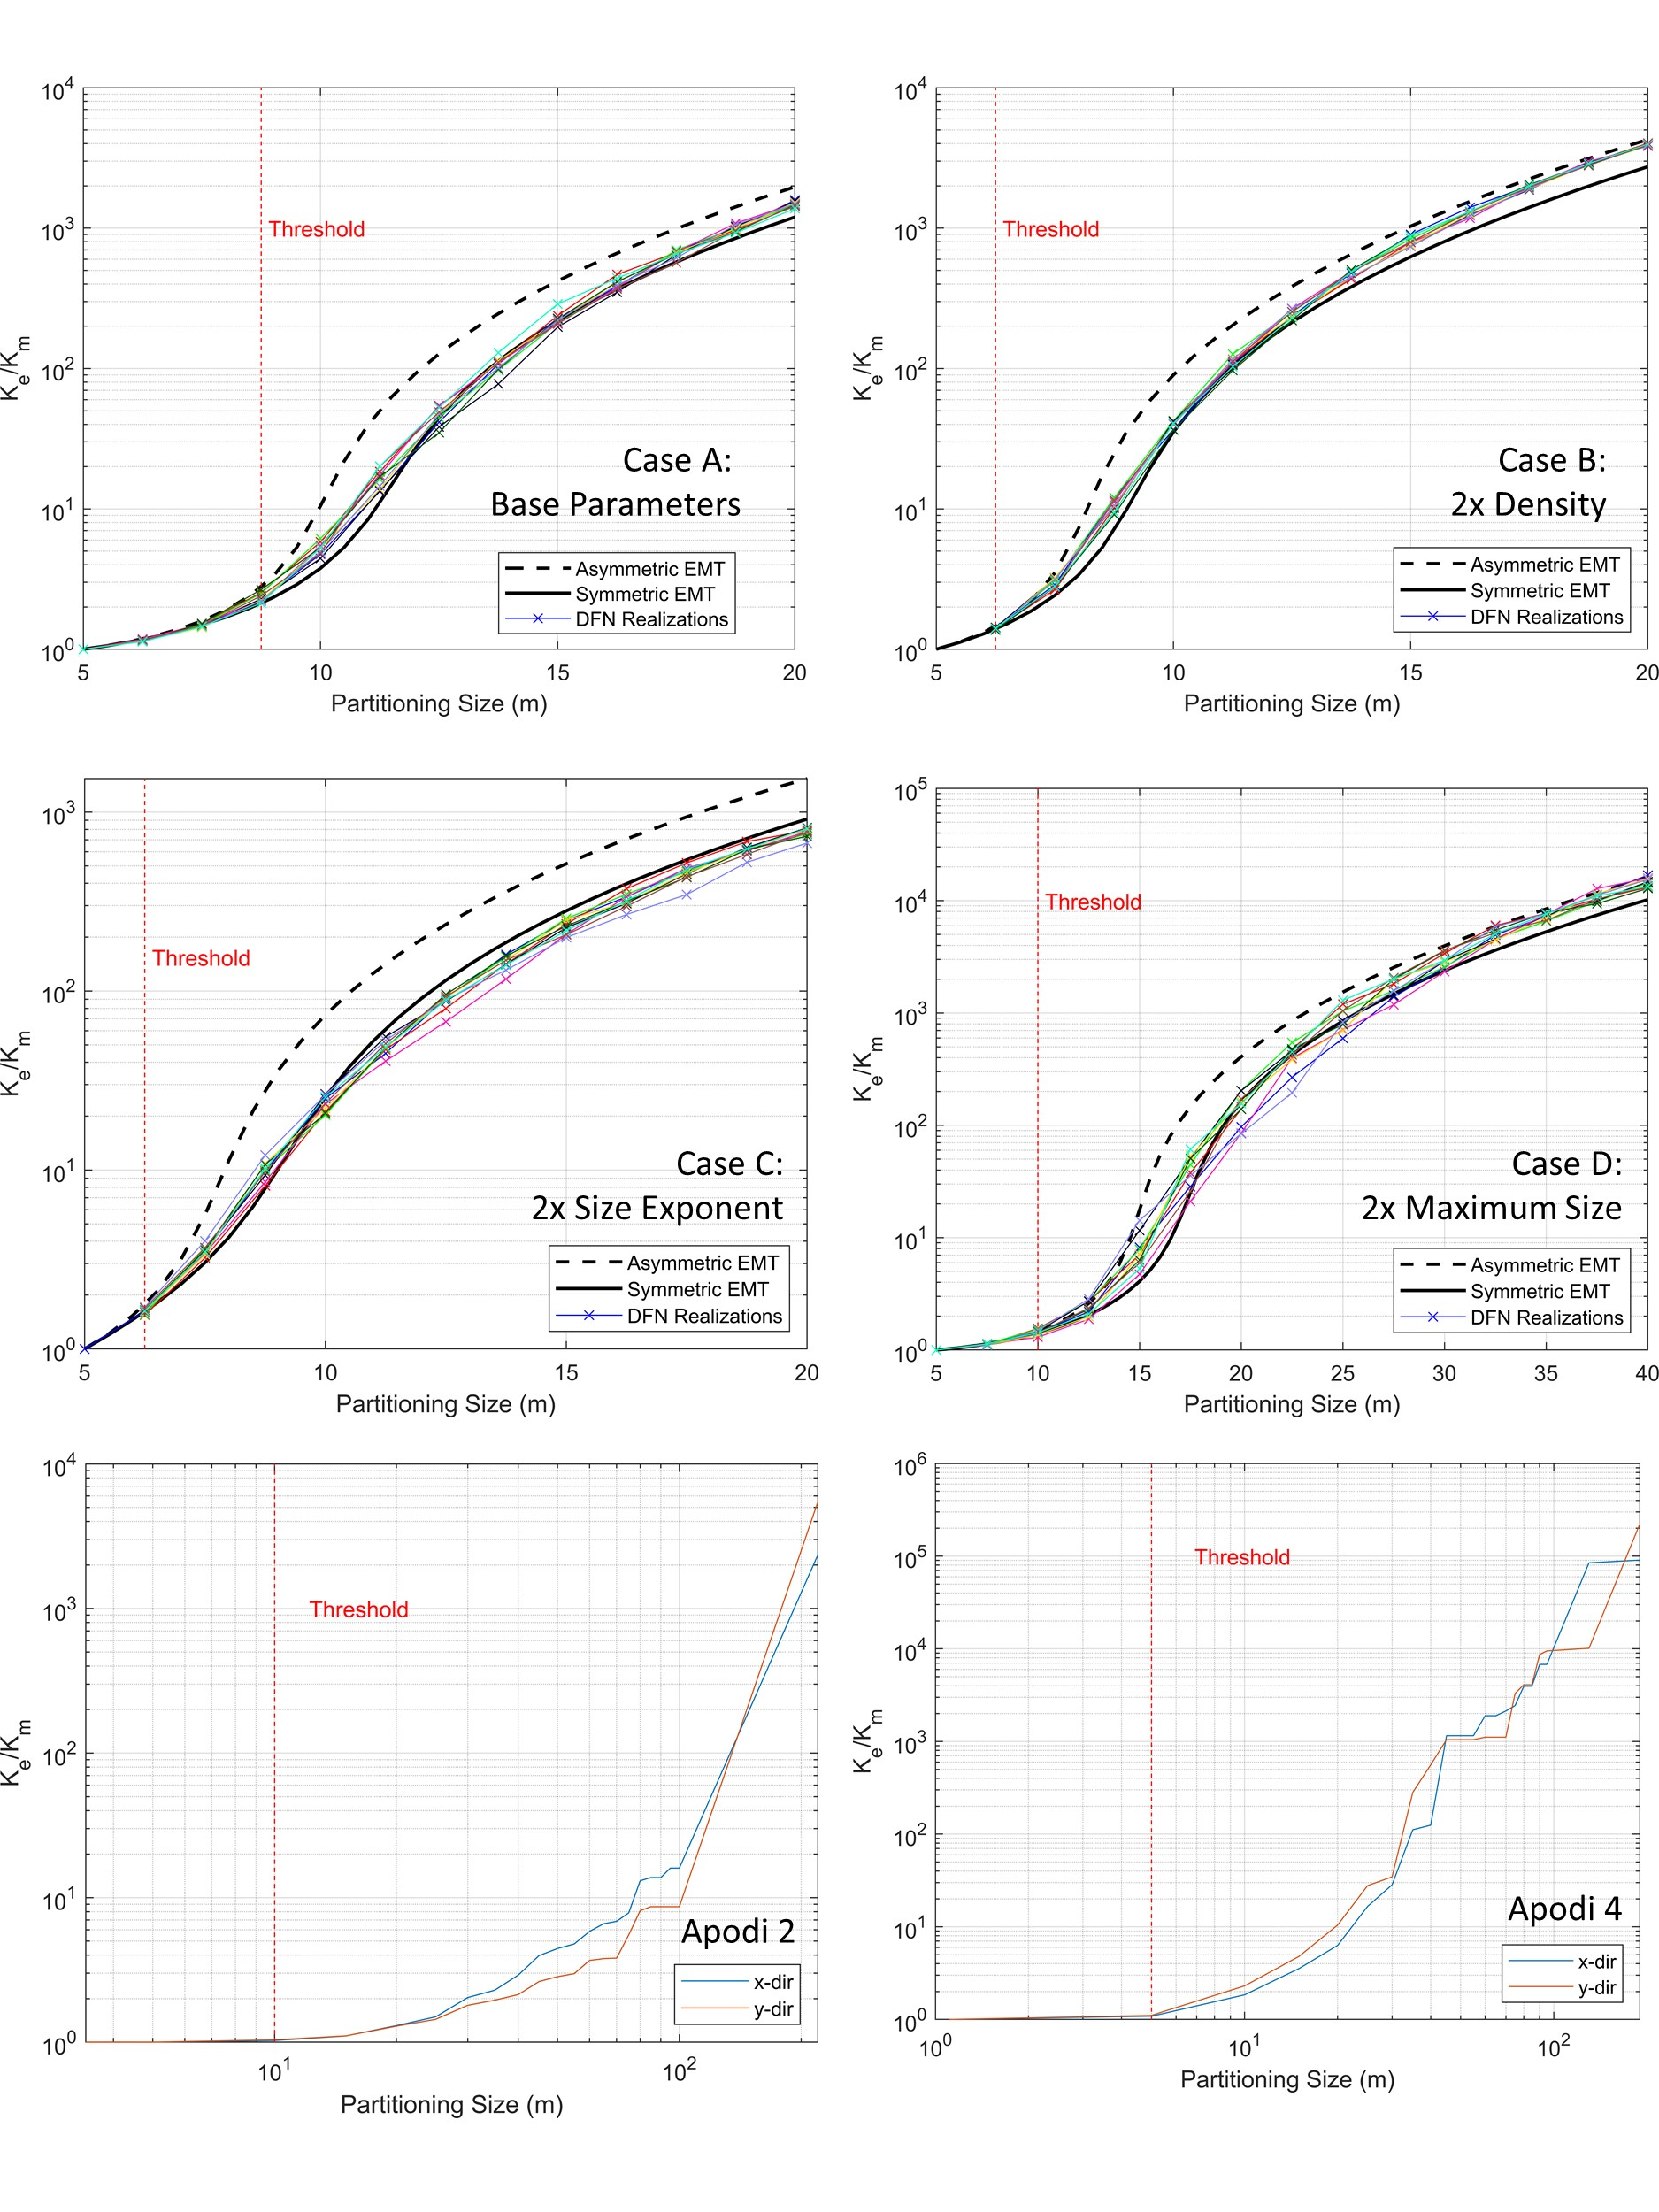
\includegraphics[width=\textwidth]{FSU_main_V.jpg}

 \caption{Fracture Subset Upscaling. Cases A to D correspond to generated 3D DFNs. 10 stochastic realizations are shown for each case to illustrate variations due to the power law size distribution used. Apodi 2 and 4 are based on outcrop fracture data. Partitioning sizes that are above the labelled threshold produce hybrid models that are inaccurate according to Figure \ref{fig:DD}.}
 \label{fig:FSU}
\end{figure}

\subsection{Single Phase Flow in Hybrid Models}
In Figure \ref{fig:DD}, we show the results for six drawdown studies based on our datasets. We further performed eleven drawdown studies that are shown in Figures S2 and S3. In all studies, we show full model solutions based on the original non-upscaled data; these serve as reference solutions. All other solutions are generated from hybrid models corresponding to different $s_p$ values. 

A fixed pressure boundary ($50$ bars) is used to initiate a drawdown for the 3D DFNs. Hence the plots show outlet flowrate against time. Due to the high fracture-to-rock permeability ratio, the pressure drop preferentially diffuses through the fracture network. When pressure in the fractures depletes significantly, fluid in the rock matrix begins to recharge the fracture network. This results in a stationary flow regime (Cases A to D in Figure \ref{fig:DD}, and Figure S2). Finally, when pressure in the entire model depletes, flowrate at the outlet goes to zero.

For Apodi 2 (Figure \ref{fig:DD}), a well is positioned in the rock matrix and drawn down at a fixed rate ($0.1$m\textsuperscript{3}/day). The pressure derivative response initially shows a straight line due to the wellbore storage effect as pressure is depleted in the well. We then observe an infinite acting regime when the perturbation at the well only diffuses through the matrix; this corresponds to the flat plateau in the derivative plot. Once the effect of the well drawdown reaches the nearest fracture, fluid depletion from the fracture network dominates due to the high fracture conductivities. This results in a dip on the pressure derivative \citep{Bourdet1989, Egya2018}. For Apodi 4, the behaviour is similar (Figure S3).

In another test, we positioned a well to intersect the largest fracture in Apodi 4 and drew down at a fixed rate ($1$m\textsuperscript{3}/day) (Figure \ref{fig:DD}). In this setup, there is similarly an initial wellbore storage effect which manifests itself in a straight line. The pressure drop at the well then diffuses through the fracture network. In this regime, the rock matrix is effectively impermeable. Once the pressure diffusion reaches the boundaries, fluid pressure in the fractures begin to drop significantly. The fluid contained in the rock matrix then begins to recharge the fracture network. This results in a dip on the pressure derivative as well \citep{Gringarten1987}. For Apodi 2, the behaviour is similar (Figure S3).

In all drawdown studies, the differences between hybrid and full model results are minimal for small $s_p$ values. This ascertains that hybrid models do have the capability to simplify simulations while preserving accuracy. However, it is observed that as $s_p$ increases, the corresponding hybrid model produces results that deviate more from the reference solution. This suggests a trade-off relationship between model simplicity and accuracy. Large $s_p$ values result in simpler models with less explicit fractures that produce less accurate results. In practice, we seek an intermediate $s_p$ which allows us to balance both needs. This will be discussed in Section \ref{discussion}.

\begin{figure}[h]
	\centering
	
	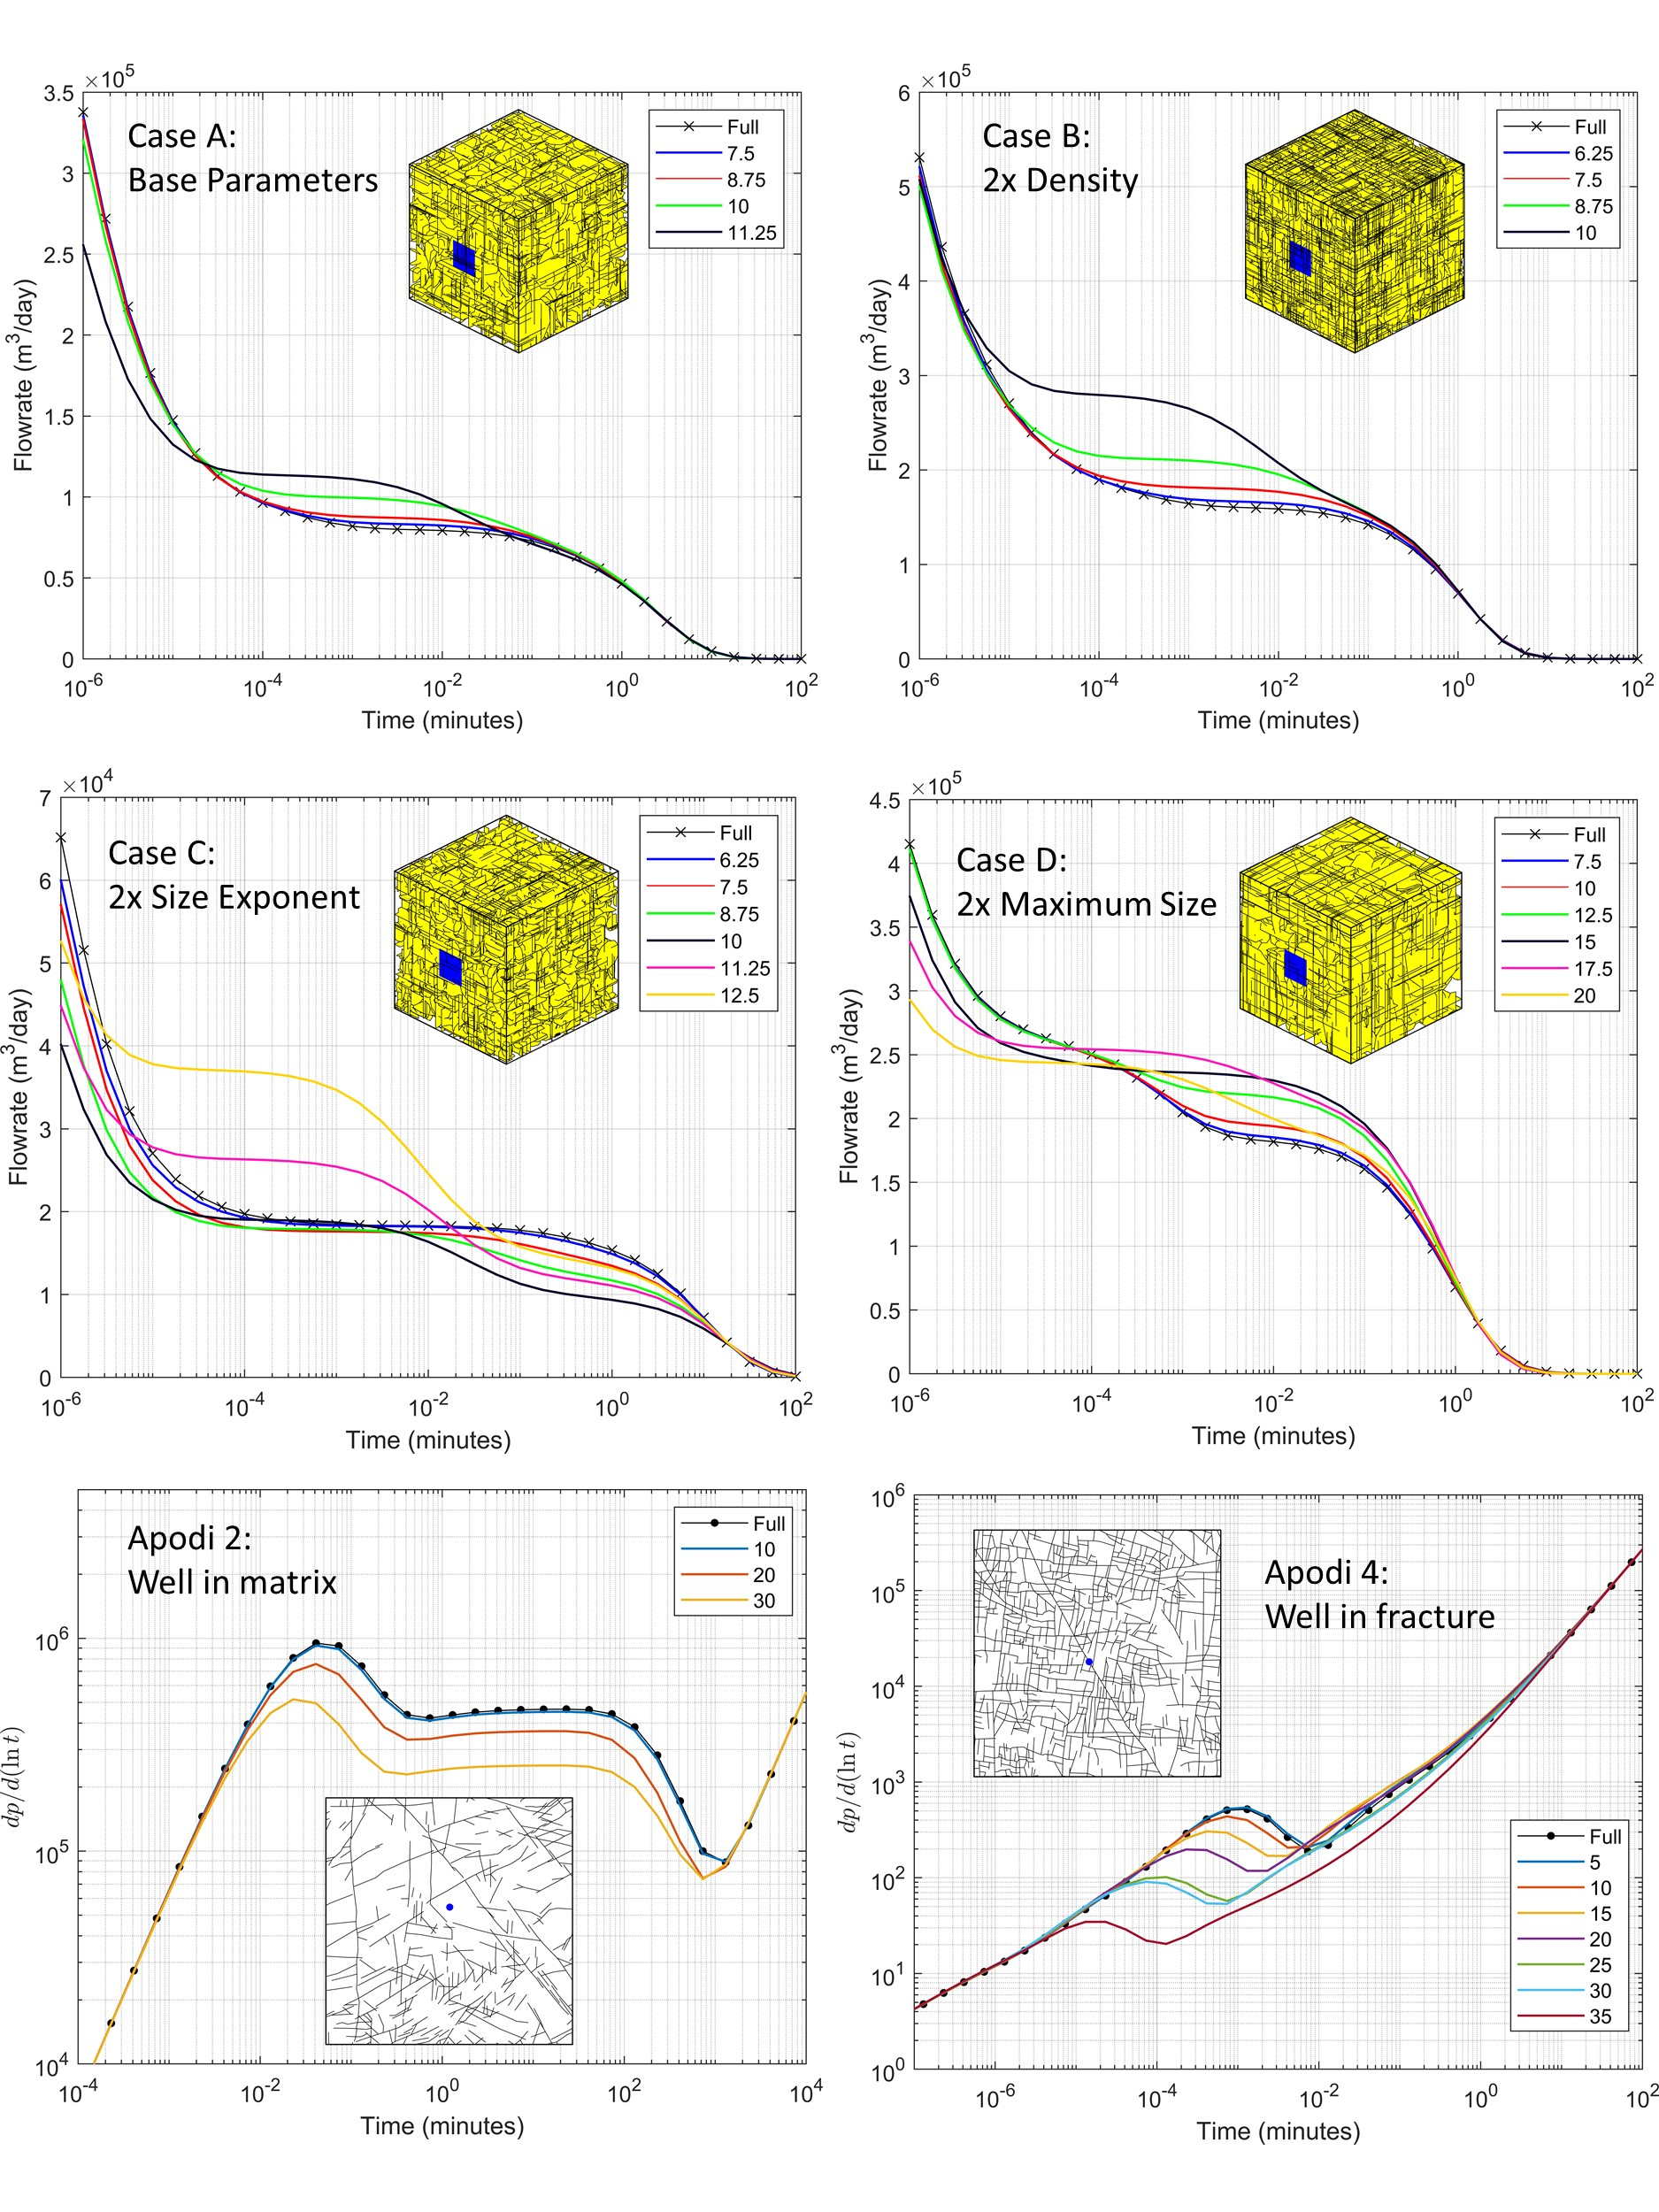
\includegraphics[width=\textwidth]{DD_main_V.jpg}
	
	\caption{Drawdown curves for fully resolved models, and hybrid models corresponding to different partitioning sizes. Cases A to D: One full DFN realization is used per case. Fixed pressure is applied on blue faces. Domain size is 100m x 100m x 100m in all cases. Apodi 2 and 4: Fixed flowrate is applied at locations marked with blue circle. Domain size is 220m x 220m x 1m and 100m x 100m x 1m for Apodi 2 and 4 respectively.}
	\label{fig:DD}
\end{figure}

\subsection{Accuracy of Effective Medium Theory}
The FSU curves generated for the 3D DFNs using the Effective Medium Theory are also shown in Figures \ref{fig:FSU} and S1. In general, there is a good match between the results obtained from both numerical and analytical approaches. We observe that the symmetric self-consistent method performs best in terms of overall $K_e$ calculations, especially at low partitioning sizes; this is in line with \citet{Saevik2013}'s observations since we are upscaling subsets of the full fracture network. We also note that the asymmetric self-consistent method tends to over-estimates $K_e$. At high densities (Case B), however, the asymmetric self-consistent method is more accurate at high $s_p$ values.

The ability of the Effective Medium Theory to capture the percolation behaviour in the FSU curves is noteworthy since its mathematical formulation does not account for fracture network topology. This has similarly been observed by \citet{Saevik2013} and no explanation has been provided yet.

The main limitation that prevents the Effective Medium Theory from being used for the Apodi 2 and 4 datasets is that it does not take into consideration the abutment relationships between fracture sets. However, in our studies, the Effective Medium Theory is significantly more efficient than numerical flow based upscaling and reduces the FSU processing time from hours to seconds.

\section{Discussion}
\label{discussion}
\subsection{Effect of Partitioning Size on Accuracy of Simulation Results}
Using the drawdown studies, we established that there is a trade-off between model simplicity and accuracy. As such, we seek an intermediate $s_p$ value that strikes a balance between the two. To this end, we further observe in Figures \ref{fig:DD}, S2 and S3 that the deviations resulting from upscaling increase abruptly as $s_p$ is increased. Hybrid models created with small $s_p$ produce drawdown results that are very similar to the corresponding full model responses. However, above a threshold partitioning size $s_p^*$, the hybrid models begin to produce results with large deviations.

The percolation behaviour in the permeability-size relationships is in line with our understanding that in order for a single porosity representation to be valid, we have to ensure that there is no separation of scale between fluid flow in the matrix and the upscaled fracture network \citep{Matthai2004a}. For low $s_p$ values, the small fractures are disperse and poorly connected. Pressure perturbations diffuse through the rock matrix and small fractures at almost equal rates. However, for high $s_p$ values, the small fractures are abundant and become well connected. In this case, pressure perturbations will preferentially diffuse through the small fractures before affecting the fluid in the rock. $s_p^*$ is the threshold where the small fractures begin to be connected. Therefore, $s_p$ must be smaller than $s_p^*$ to obtain an accurate single porosity hybrid model.

From a pragmatic viewpoint, a threshold partitioning size $s_p^*$ implies a limit to how much we can simplify our simulation model. This is because as $s_p$ increases beyond $s_p^*$, we begin to reduce computational load at the expense of model accuracy. In practice, determining $s_p^*$ allows us to assess our modelling approach. If the simulation grid size used in a model is smaller than $s_p^*$, we can be sure that upscaling fractures smaller than the grid cell will not negatively impact model accuracy.


\subsection{\textit{A priori} Identification of Partitioning Threshold}
So far, we have identified partitioning thresholds $s_p^*$ based on comparisons of drawdown simulation results. This requires performing FSU across a range of $s_p$ values and creating a series of hybrid models. The models are then subjected to drawdown simulations and their results are compared in order to identify $s_p^*$.

In practice, this is a time consuming process and will not be useful. Instead, we can identify $s_p^*$ \textit{a priori} by exploiting the percolation behaviour observed in the FSU curves. We recall that when small fractures are poorly connected, we expect FSU to produce low $K_e/K_m$ values, vice versa. Since a single porosity hybrid model requires small fractures to be poorly connected, the threshold for $s_p$ corresponds to where $K_e/K_m$ begins to increase rapidly. To illustrate this, the values of $s_p^*$ as identified from our drawdown simulation results have been marked out on the FSU curves in Figures \ref{fig:FSU} and S1. The results show that FSU curves can indeed be used to determine threshold partitioning sizes without running any production simulations.

The process of identifying $s_p^*$ can be further expedited with the help of the Effective Medium Theory. As was shown in Figures \ref{fig:FSU} and S1, for uncorrelated fracture sets, with fractures uniformly distributed in space, performing FSU with the Effective Medium Theory yields results that match numerical flow based upscaling. However, since the Effective Medium Theory is a semi-analytical upscaling tool, it produces results in seconds rather than hours. In reality, fracture networks may be less conductive than predicted by the theory. This is because fracture sets are usually correlated with each other through abutment relationships. This correlation results in less intersections per fracture than expected. Research is ongoing to incorporate such relationships in analytical upscaling tools \citep{Hardebol2015, Makel2007, Saevik2017}. 

\section{Conclusion}
Fluid flow modelling in naturally fractured reservoirs is a challenging process due to the multiscale nature of fractures. One of the major difficulties is the accurate representation of multiscale fractures in simulation models. Single porosity hybrid models that represent small fractures implicitly and large fractures explicitly are useful in this regard. Splitting a fracture set into small and large sets requires the choice of a partitioning size.

We conducted numerical studies using synthetic 3D and outcrop based 2D datasets. The drawdown simulations performed on full non-upscaled, and hybrid models confirm that hybrid models created with partitioning sizes do reduce simulation complexity while maintaining accuracy of outputs. However, partitioning sizes must not be unreasonably large. In fact, for each dataset, we identified a threshold partitioning size beyond which single porosity hybrid models become significantly inaccurate.

For every dataset, we can identify the threshold partitioning size by solving the Laplace equation either numerically or analytically. By upscaling small fractures with the rock matrix, we obtain effective permeabilities that depend on partitioning size. This permeability-size relationship is also referred to as a Fracture Subset Upscaling curve. The threshold partitioning size coincides with the point on the curve where effective permeability of small fractures begins to increase significantly. 

Finally, we also note that Fracture Subset Upscaling can be performed \textit{a priori} and efficiently using the Effective Medium Theory, which is a semi-analytical upscaling tool. This technique reduces the time needed to generate the permeability-size relationship from hours to seconds. However, the Effective Medium Theory currently does not take into consideration geological features such as abutment relationships and non-uniform spatial distributions of fractures. Where necessary, numerical flow based upscaling can also be used for Fracture Subset Upscaling. In terms of fracture network properties, a numerical approach is less restrictive, but is significantly more resource intensive.
%Text here ===>>>

%%

%  Numbered lines in equations:
%  To add line numbers to lines in equations,
%  \begin{linenomath*}
%  \begin{equation}
%  \end{equation}
%  \end{linenomath*}



%% Enter Figures and Tables near as possible to where they are first mentioned:
%
% DO NOT USE \psfrag or \subfigure commands.
%
% Figure captions go below the figure.
% Table titles go above tables;  other caption information
%  should be placed in last line of the table, using
% \multicolumn2l{$^a$ This is a table note.}
%
%----------------
% EXAMPLE FIGURE
%
% \begin{figure}[h]
% \centering
% when using pdflatex, use pdf file:
% \includegraphics[natwidth=800px,natheight=600px]{figsamp.pdf}
%
% when using dvips, use .eps file:
% \includegraphics[natwidth=800px,natheight=600px]{figsamp.eps}
%
% \caption{Short caption}
% \label{figone}
%  \end{figure}
%
% We recommend that you provide the native width and height (natwidth, natheight) of your figures.
% Specifying native dimensions ensures that your figures are properly scaled
%
%
% ---------------
% EXAMPLE TABLE
%
% \begin{table}
% \caption{Time of the Transition Between Phase 1 and Phase 2$^{a}$}
% \centering
% \begin{tabular}{l c}
% \hline
%  Run  & Time (min)  \\
% \hline
%   $l1$  & 260   \\
%   $l2$  & 300   \\
%   $l3$  & 340   \\
%   $h1$  & 270   \\
%   $h2$  & 250   \\
%   $h3$  & 380   \\
%   $r1$  & 370   \\
%   $r2$  & 390   \\
% \hline
% \multicolumn{2}{l}{$^{a}$Footnote text here.}
% \end{tabular}
% \end{table}

%% SIDEWAYS FIGURE and TABLE
% AGU prefers the use of {sidewaystable} over {landscapetable} as it causes fewer problems.
%
% \begin{sidewaysfigure}
% \includegraphics[width=20pc]{figsamp}
% \caption{caption here}
% \label{newfig}
% \end{sidewaysfigure}
%
%  \begin{sidewaystable}
%  \caption{Caption here}
% \label{tab:signif_gap_clos}
%  \begin{tabular}{ccc}
% one&two&three\\
% four&five&six
%  \end{tabular}
%  \end{sidewaystable}

%% If using numbered lines, please surround equations with \begin{linenomath*}...\end{linenomath*}
%\begin{linenomath*}
%\begin{equation}
%y|{f} \sim g(m, \sigma),
%\end{equation}
%\end{linenomath*}

%%% End of body of article

%%%%%%%%%%%%%%%%%%%%%%%%%%%%%%%%
%% Optional Appendix goes here
%
% The \appendix command resets counters and redefines section heads
%
% After typing \appendix
%
%\section{Here Is Appendix Title}
% will show
% A: Here Is Appendix Title
%
%\appendix
%\section{Here is a sample appendix}

%%%%%%%%%%%%%%%%%%%%%%%%%%%%%%%%%%%%%%%%%%%%%%%%%%%%%%%%%%%%%%%%
%
% Optional Glossary, Notation or Acronym section goes here:
%
%%%%%%%%%%%%%%
% Glossary is only allowed in Reviews of Geophysics
%  \begin{glossary}
%  \term{Term}
%   Term Definition here
%  \term{Term}
%   Term Definition here
%  \term{Term}
%   Term Definition here
%  \end{glossary}

%
%%%%%%%%%%%%%%
% Acronyms
%   \begin{acronyms}
%   \acro{Acronym}
%   Definition here
%   \acro{EMOS}
%   Ensemble model output statistics
%   \acro{ECMWF}
%   Centre for Medium-Range Weather Forecasts
%   \end{acronyms}

%
%%%%%%%%%%%%%%
% Notation
%   \begin{notation}
%   \notation{$a+b$} Notation Definition here
%   \notation{$e=mc^2$}
%   Equation in German-born physicist Albert Einstein's theory of special
%  relativity that showed that the increased relativistic mass ($m$) of a
%  body comes from the energy of motion of the body—that is, its kinetic
%  energy ($E$)—divided by the speed of light squared ($c^2$).
%   \end{notation}




%%%%%%%%%%%%%%%%%%%%%%%%%%%%%%%%%%%%%%%%%%%%%%%%%%%%%%%%%%%%%%%%
%
%  ACKNOWLEDGMENTS
%
% The acknowledgments must list:
%
% >>>>	A statement that indicates to the reader where the data
% 	supporting the conclusions can be obtained (for example, in the
% 	references, tables, supporting information, and other databases).
%
% 	All funding sources related to this work from all authors
%
% 	Any real or perceived financial conflicts of interests for any
%	author
%
% 	Other affiliations for any author that may be perceived as
% 	having a conflict of interest with respect to the results of this
% 	paper.
%
%
% It is also the appropriate place to thank colleagues and other contributors.
% AGU does not normally allow dedications.


\acknowledgments
The authors are grateful to Total, S.A. for funding Daniel Wong's PhD research. We also thank Energi Simulation for funding Sebastian Geiger's Chair in Carbonate Reservoir Simulation. Finally, we thank TU Delft for making their datasets available through \citet{Bisdom2017}.


%% ------------------------------------------------------------------------ %%
%% References and Citations

%%%%%%%%%%%%%%%%%%%%%%%%%%%%%%%%%%%%%%%%%%%%%%%
% BibTeX is preferred:
%
% \bibliography{<name of your .bib file>}
%
% don't specify bibliographystyle
%%%%%%%%%%%%%%%%%%%%%%%%%%%%%%%%%%%%%%%%%%%%%%%

\bibliography{library}

% Please use ONLY \citet and \citep for reference citations.
% DO NOT use other cite commands (e.g., \cite, \citeyear, \nocite, \citealp, etc.).
%% Example \citet and \citep:
%  ...as shown by \citet{Boug10}, \citet{Buiz07}, \citet{Fra10},
%  \citet{Ghel00}, and \citet{Leit74}.

%  ...as shown by \citep{Boug10}, \citep{Buiz07}, \citep{Fra10},
%  \citep{Ghel00, Leit74}.

%  ...has been shown \citep [e.g.,][]{Boug10,Buiz07,Fra10}.


\end{document}



More Information and Advice:

%% ------------------------------------------------------------------------ %%
%
%  SECTION HEADS
%
%% ------------------------------------------------------------------------ %%

% Capitalize the first letter of each word (except for
% prepositions, conjunctions, and articles that are
% three or fewer letters).

% AGU follows standard outline style; therefore, there cannot be a section 1 without
% a section 2, or a section 2.3.1 without a section 2.3.2.
% Please make sure your section numbers are balanced.
% ---------------
% Level 1 head
%
% Use the \section{} command to identify level 1 heads;
% type the appropriate head wording between the curly
% brackets, as shown below.
%
%An example:
%\section{Level 1 Head: Introduction}
%
% ---------------
% Level 2 head
%
% Use the \subsection{} command to identify level 2 heads.
%An example:
%\subsection{Level 2 Head}
%
% ---------------
% Level 3 head
%
% Use the \subsubsection{} command to identify level 3 heads
%An example:
%\subsubsection{Level 3 Head}
%
%---------------
% Level 4 head
%
% Use the \subsubsubsection{} command to identify level 3 heads
% An example:
%\subsubsubsection{Level 4 Head} An example.
%
%% ------------------------------------------------------------------------ %%
%
%  IN-TEXT LISTS
%
%% ------------------------------------------------------------------------ %%
%
% Do not use bulleted lists; enumerated lists are okay.
% \begin{enumerate}
% \item
% \item
% \item
% \end{enumerate}
%
%% ------------------------------------------------------------------------ %%
%
%  EQUATIONS
%
%% ------------------------------------------------------------------------ %%

% Single-line equations are centered.
% Equation arrays will appear left-aligned.

Math coded inside display math mode \[ ...\]
 will not be numbered, e.g.,:
 \[ x^2=y^2 + z^2\]

 Math coded inside \begin{equation} and \end{equation} will
 be automatically numbered, e.g.,:
 \begin{equation}
 x^2=y^2 + z^2
 \end{equation}


% To create multiline equations, use the
% \begin{eqnarray} and \end{eqnarray} environment
% as demonstrated below.
\begin{eqnarray}
  x_{1} & = & (x - x_{0}) \cos \Theta \nonumber \\
        && + (y - y_{0}) \sin \Theta  \nonumber \\
  y_{1} & = & -(x - x_{0}) \sin \Theta \nonumber \\
        && + (y - y_{0}) \cos \Theta.
\end{eqnarray}

%If you don't want an equation number, use the star form:
%\begin{eqnarray*}...\end{eqnarray*}

% Break each line at a sign of operation
% (+, -, etc.) if possible, with the sign of operation
% on the new line.

% Indent second and subsequent lines to align with
% the first character following the equal sign on the
% first line.

% Use an \hspace{} command to insert horizontal space
% into your equation if necessary. Place an appropriate
% unit of measure between the curly braces, e.g.
% \hspace{1in}; you may have to experiment to achieve
% the correct amount of space.


%% ------------------------------------------------------------------------ %%
%
%  EQUATION NUMBERING: COUNTER
%
%% ------------------------------------------------------------------------ %%

% You may change equation numbering by resetting
% the equation counter or by explicitly numbering
% an equation.

% To explicitly number an equation, type \eqnum{}
% (with the desired number between the brackets)
% after the \begin{equation} or \begin{eqnarray}
% command.  The \eqnum{} command will affect only
% the equation it appears with; LaTeX will number
% any equations appearing later in the manuscript
% according to the equation counter.
%

% If you have a multiline equation that needs only
% one equation number, use a \nonumber command in
% front of the double backslashes (\\) as shown in
% the multiline equation above.

% If you are using line numbers, remember to surround
% equations with \begin{linenomath*}...\end{linenomath*}

%  To add line numbers to lines in equations:
%  \begin{linenomath*}
%  \begin{equation}
%  \end{equation}
%  \end{linenomath*}



